\documentclass{article}
\usepackage[utf8]{inputenc}

\title{Guía de Estilo de la revista Laberintos e Infinitos}
\author{Equipo editorial de Laberintos e Infinitos}
\date{Julio 2018}

\usepackage{graphicx}
\usepackage{hyperref}

\begin{document}

\maketitle

\section{Puntos Generales}
La revista Laberintos e Infinitos intenta ser una revista de nivel medio que publica artículos académicos. Estos artículos son parte de las áreas generales de estudio de Matemáticas y Actuaria. Lo que esto significa es que los artículos generalmente serán de nivel de licenciatura. Se aceptan artículos de cualquier persona sin discriminación por cualquier motivo, pero a veces se le da preferencia personas de la comunidad ITAM, siendo esta revista creada por ellos y principalmente para esta comunidad. 

\section{Paleta de Colores}

Los colores utilizados en el diseño general de la revista son los siguientes: 
\begin{figure}[h!]
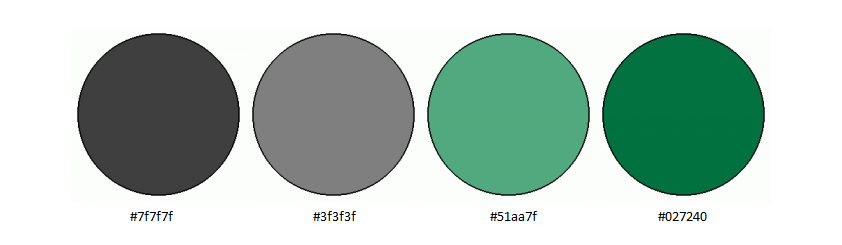
\includegraphics[width=15cm]{paleta.png}
\centering
\end{figure}

Al generar gráficas o presentar resultados de una forma visual, se le pide al autor considerar estos colores como la base para poder mantener consistencia visual dentro de toda la revista. Considérese que la revista es en su mayoría en blanco y negro menos en su publicación como pdf en linea, entonces colores claros pueden llevar a problemas con la presentación de información. 

% Me encantaria poner un ejemplo aqui. 



\section{Tipografía}

Se usa en la revista el tipo de fase de quattrocento. Es uno de los fonts incluidos en LaTeX, entonces se puede conseguir junto con el template de la revista en laberintos.itam.mx. En otro caso, por favor contactar a alguno de los editores de la revista, ya que todos tienen acceso a el. Se usa también el estilo $\textnormal{amsmath}$ para la presentación de ecuaciones y todo lo escrito en el incluido \textit{math mode} de LaTex. 

\begin{figure}[ht]

\includegraphics[width=12cm]{font.png}
\centering
\end{figure}

\subsection{Espaciado}
Se usa espaciado de 1.2 entre todas las lineas, esto por claridad. 

\section{Codigo y Algoritmos} 
Al utilizar código en el articulo, se utiliza en la revista el paquete de LaTex de lstlisting. Se pide además que al importar el código usando el paquete, se utilice el lenguaje en el que esta escrito, para tener resaltado de texto y espacio de lineas como en el código original. 

Un tema separado es el uso de algoritmos sin código explicito, y en este caso, utilizamos internamente el paquete de algorith2e.

\section{Citas}
Al citar alguna fuente de información utilizada en el articulo, usamos la guía de Chicago. Se puede encontrar mas información buscando \textit{Chicago Manual of Style} en linea o en la siguiente pagina: \href{http://www.chicagomanualofstyle.org/tools_citationguide/citation-guide-1.html}{\underline{Chicago Manual of Style - Citation}}.








\end{document}
